\documentclass[12pt,a4paper]{article}

% ─── Packages ────────────────────────────────────────────────────────────
\usepackage[utf8]{inputenc}
\usepackage[T1]{fontenc}
\usepackage{lmodern}
\usepackage[margin=1in]{geometry}
\usepackage{graphicx}
\usepackage{tikz}
\usetikzlibrary{shapes.geometric, arrows.meta, positioning, fit, calc, backgrounds, decorations.pathreplacing}
\usepackage{pgfplots}
\pgfplotsset{compat=1.18}
\usepackage{booktabs}
\usepackage{array}
\usepackage{tabularx}
\usepackage{hyperref}
\usepackage{xcolor}
\usepackage{enumitem}
\usepackage{titlesec}
\usepackage{fancyhdr}
\usepackage{setspace}
\usepackage{caption}
\usepackage{float}

% ─── Colors ──────────────────────────────────────────────────────────────
\definecolor{primary}{RGB}{225,29,72}
\definecolor{secondary}{RGB}{13,148,136}
\definecolor{accent}{RGB}{245,158,11}
\definecolor{dark}{RGB}{15,23,42}
\definecolor{lightgray}{RGB}{241,245,249}
\definecolor{midgray}{RGB}{148,163,184}
\definecolor{success}{RGB}{16,185,129}
\definecolor{danger}{RGB}{239,68,68}
\definecolor{linkblue}{RGB}{37,99,235}

\hypersetup{
    colorlinks=true,
    linkcolor=linkblue,
    urlcolor=linkblue,
    citecolor=linkblue,
}

% ─── Header / Footer ────────────────────────────────────────────────────
\pagestyle{fancy}
\fancyhf{}
\fancyhead[L]{\small\textcolor{midgray}{LifeLink --- Blood \& Organ Donor Matching System}}
\fancyhead[R]{\small\textcolor{midgray}{IEEE Project Documentation}}
\fancyfoot[C]{\small\textcolor{midgray}{\thepage}}
\renewcommand{\headrulewidth}{0.4pt}

% ─── Section Formatting ─────────────────────────────────────────────────
\titleformat{\section}{\Large\bfseries\color{dark}}{}{0em}{}[\color{primary}\titlerule]
\titleformat{\subsection}{\large\bfseries\color{dark}}{}{0em}{}
\titleformat{\subsubsection}{\normalsize\bfseries\color{dark}}{}{0em}{}

\onehalfspacing

% ══════════════════════════════════════════════════════════════════════════
\begin{document}

% ─── Title Page ──────────────────────────────────────────────────────────
\begin{titlepage}
    \centering
    \vspace*{2cm}

    % Logo
    
\begin{tikzpicture}
        \shade[inner color=primary!90, outer color=primary!60]
            (0,0) .. controls (0,1.2) and (1.5,3) .. (1.5,3)
            .. controls (1.5,3) and (3,1.2) .. (3,0)
            .. controls (3,-0.8) and (2.2,-1.5) .. (1.5,-1.5)
            .. controls (0.8,-1.5) and (0,-0.8) .. (0,0) -- cycle;
        \draw[white, line width=1.5pt, line cap=round]
            (0.7,0.8) -- (1.0,-0.2) -- (1.3,1.2) -- (1.6,-0.2) -- (1.9,0.8);
    \end{tikzpicture}

    \vspace{1cm}
    {\Huge\bfseries\textcolor{dark}{LifeLink} \par}
    \vspace{0.3cm}
    {\Large\textcolor{primary}{Blood and Organ Donor Matching System} \par}
    \vspace{0.5cm}
    {\large\textcolor{midgray}{An IEEE Project} \par}

    \vspace{3cm}

    % Team Members Table
    {\large\textcolor{dark}{Team Members} \par}
    \vspace{0.5cm}
    \renewcommand{\arraystretch}{1.6}
    \begin{tabular}{|>{\centering\arraybackslash}m{0.4\textwidth}|>{\centering\arraybackslash}m{0.4\textwidth}|}
        \hline
        \textbf{Name} & \textbf{Contribution} \\
        \hline
        Amiya Bar & Frontend Development \\
        \hline
        Dhanush Pillay & Backend \& Database \\
        \hline
        Krish Bansod & UI/UX \& Integration \\
        \hline
        Shubhangini Dixit & Research \& Documentation \\
        \hline
    \end{tabular}

    \vspace{3cm}

    {\large\textcolor{dark}{\today} \par}
    \vfill
    {\small\textcolor{midgray}{Department of Computer Science and Engineering} \par}
    {\small\textcolor{midgray}{Developed for IEEE Project Submission} \par}
\end{titlepage}

% ─── Table of Contents ───────────────────────────────────────────────────
\newpage
\tableofcontents
\newpage

% ══════════════════════════════════════════════════════════════════════════
% SECTION 1: ABSTRACT
% ══════════════════════════════════════════════════════════════════════════
\section{Abstract}

LifeLink is a web-based platform designed to connect blood and organ donors with patients and hospitals during medical emergencies. The system allows users to register as donors, search for compatible donors in real-time based on blood group, organ type, and geographic proximity, and communicate securely through built-in chat and masked calling features. Built using the MERN stack (MongoDB, Express.js, React.js, Node.js) with real-time Server-Sent Events for live notifications, the platform aims to reduce emergency response time, support rare blood group matching, and promote ethical donor management through a transparent, privacy-first digital ecosystem.

\textbf{Keywords:} Donor Matching, Blood Donation, Organ Donation, Real-Time Notifications, MERN Stack, Location-Based Search, Emergency Healthcare

% ══════════════════════════════════════════════════════════════════════════
% SECTION 2: INTRODUCTION
% ══════════════════════════════════════════════════════════════════════════
\section{Introduction}

\subsection{What is LifeLink?}

LifeLink is a website that helps people find blood and organ donors when they need them the most. Think of it like a \textbf{search engine for saving lives} --- you type in the blood group you need (like O+ or A-), and the system shows you verified donors nearby who are available to donate.

\subsection{Why was it built?}

During medical emergencies, every second counts. Currently, patients and hospitals struggle to find compatible donors quickly. The process is often manual, slow, and lacks transparency. LifeLink solves this by providing:

\begin{itemize}[leftmargin=*]
    \item \textbf{Instant Search} --- Find donors in seconds based on blood group and location
    \item \textbf{Real-Time Alerts} --- Matching donors get notified immediately through the app
    \item \textbf{Privacy Protection} --- Personal details are hidden until the user chooses to connect
    \item \textbf{Emergency Support} --- Critical requests are broadcast to all matching donors in a city
    \item \textbf{Secure Communication} --- Built-in chat and masked calling protect both parties
\end{itemize}

\subsection{Who uses it?}

\begin{enumerate}[leftmargin=*]
    \item \textbf{Donors} --- People who want to register as blood or organ donors and set their availability
    \item \textbf{Hospitals} --- Healthcare facilities that post donation requests and get auto-matched with donors
    \item \textbf{Patients / General Users} --- Anyone looking for a compatible donor for themselves or someone they know
\end{enumerate}

% ══════════════════════════════════════════════════════════════════════════
% SECTION 3: PROBLEM STATEMENT
% ══════════════════════════════════════════════════════════════════════════
\section{Problem Statement}

Finding compatible blood and organ donors during emergencies remains a significant challenge for hospitals and patients. The key problems are:

\begin{enumerate}[leftmargin=*]
    \item \textbf{Time Delay} --- Traditional methods of finding donors (word of mouth, social media posts) are slow and unreliable during critical situations.
    \item \textbf{Rare Blood Groups} --- Patients with rare blood groups (like AB-, O-) face extreme difficulty finding compatible donors.
    \item \textbf{Lack of Centralization} --- There is no single platform that connects all donors, hospitals, and patients in one place.
    \item \textbf{Privacy Concerns} --- Donors are often reluctant to share personal contact information publicly.
    \item \textbf{Illegal Organ Trafficking} --- The absence of a transparent system can lead to unethical practices.
\end{enumerate}

% ══════════════════════════════════════════════════════════════════════════
% SECTION 4: PROPOSED SOLUTION
% ══════════════════════════════════════════════════════════════════════════
\section{Proposed Solution}

LifeLink proposes a centralized web-based platform that addresses all the above problems:

\begin{enumerate}[leftmargin=*]
    \item \textbf{Donor Registration} --- Users register with medical details, blood group, and organ preferences, creating a verified donor database.
    \item \textbf{Smart Matching Algorithm} --- When a request is posted, the system automatically finds matching donors based on blood group, organ type, and city.
    \item \textbf{Emergency Broadcast} --- Critical requests instantly notify all matching donors in the city.
    \item \textbf{Location-Based Search} --- Donors are found using GPS coordinates and sorted by distance using the Haversine formula.
    \item \textbf{Privacy-First Design} --- No personal details (name, phone, email) are shown until the user explicitly chooses to connect.
    \item \textbf{Secure Communication} --- Built-in real-time chat and masked calling protect user identities.
    \item \textbf{Medical Verification} --- Donors upload medical certificates for eligibility verification.
\end{enumerate}

% ══════════════════════════════════════════════════════════════════════════
% SECTION 5: TECHNOLOGY STACK
% ══════════════════════════════════════════════════════════════════════════
\section{Technology Stack}

\begin{table}[H]
\centering
\renewcommand{\arraystretch}{1.5}
\begin{tabularx}{\textwidth}{|>{\bfseries\color{dark}}l|X|X|}
    \hline
    \textbf{Layer} & \textbf{Technology} & \textbf{Purpose} \\
    \hline
    Frontend & React 19, Vite & Component-based UI, fast development server \\
    \hline
    Routing & React Router v7 & Single-page application navigation \\
    \hline
    HTTP Client & Axios & API calls with JWT interceptor \\
    \hline
    Styling & Custom CSS (Glassmorphism) & Modern glass-effect UI design \\
    \hline
    Backend & Node.js, Express.js & REST API server, middleware pipeline \\
    \hline
    Database & MongoDB, Mongoose & NoSQL document store, schema modeling \\
    \hline
    Authentication & JWT, bcrypt, Google OAuth & Stateless auth, password hashing, social login \\
    \hline
    Validation & Joi & Request body schema validation \\
    \hline
    Real-Time & Server-Sent Events (SSE) & Live notifications, request updates \\
    \hline
    Chat & REST API & Message send/receive, typing indicators \\
    \hline
    Push Notifications & Firebase Cloud Messaging & Browser push when user is offline \\
    \hline
    Location & Geolocation API, Nominatim & GPS detection, reverse geocoding \\
    \hline
    Security & Helmet, express-rate-limit & HTTP headers, 500 req/15min limit \\
    \hline
    Deployment & Docker Compose & Containerized mongo + backend + frontend \\
    \hline
    Hosting & Vercel (Frontend) & Static deployment with auto-build \\
    \hline
\end{tabularx}
\caption{Technology Stack Overview}
\end{table}

% ══════════════════════════════════════════════════════════════════════════
% SECTION 6: SYSTEM ARCHITECTURE
% ══════════════════════════════════════════════════════════════════════════
\section{System Architecture}

The system follows a three-tier architecture: Presentation Layer (Frontend), Application Layer (Backend), and Data Layer (Database).

\begin{figure}[H]
\centering
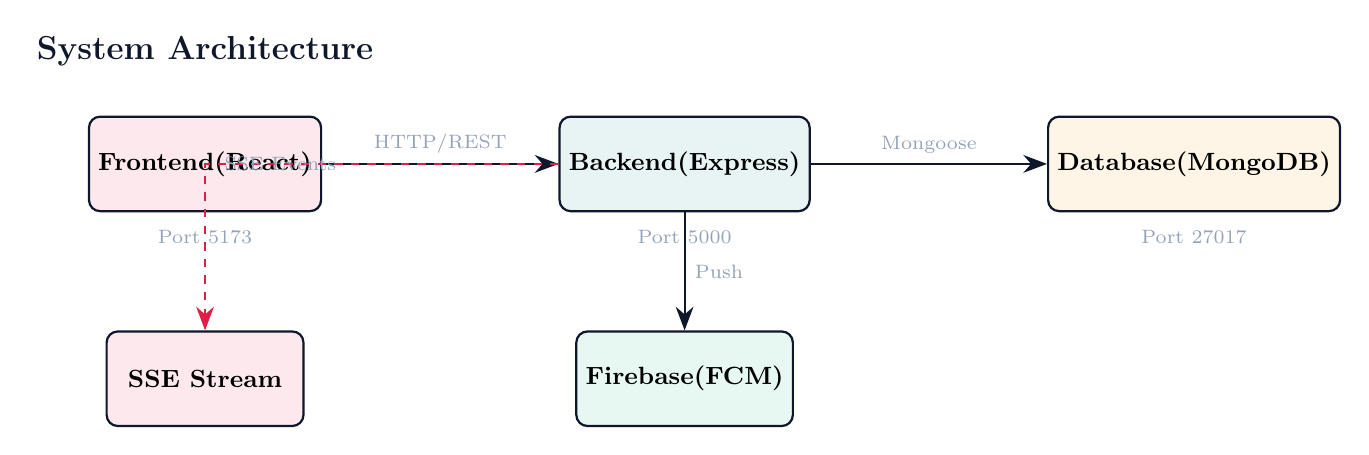
\begin{tikzpicture}[
    node distance=1.8cm and 2.5cm,
    box/.style={rectangle, rounded corners, minimum width=2.5cm, minimum height=1.2cm, text centered, font=\small\bfseries, draw=dark, line width=0.8pt},
    arrow/.style={-{Stealth[length=3mm]}, thick, dark},
    label/.style={font=\scriptsize, text=midgray},
]

% Frontend
\node[box, fill=primary!10] (frontend) {Frontend\\(React)};
\node[label, below=0.1cm of frontend] {Port 5173};

% Backend
\node[box, fill=secondary!10, right=3cm of frontend] (backend) {Backend\\(Express)};
\node[label, below=0.1cm of backend] {Port 5000};

% Database
\node[box, fill=accent!10, right=3cm of backend] (db) {Database\\(MongoDB)};
\node[label, below=0.1cm of db] {Port 27017};

% Firebase
\node[box, fill=success!10, below=1.5cm of backend] (firebase) {Firebase\\(FCM)};

% SSE Stream
\node[box, fill=primary!10, below=1.5cm of frontend] (sse) {SSE Stream};

% Arrows
\draw[arrow] (frontend) -- node[above, label] {HTTP/REST} (backend);
\draw[arrow] (backend) -- node[above, label] {Mongoose} (db);
\draw[arrow] (backend) -- node[right, label] {Push} (firebase);
\draw[arrow, dashed, primary] (backend) -| node[left, label, pos=0.3] {SSE Events} (sse);

% Title
\node[above=0.5cm of frontend, font=\large\bfseries\color{dark}] {System Architecture};

\end{tikzpicture}
\caption{Three-Tier System Architecture}
\end{figure}

\subsection{Architecture Description}

\begin{enumerate}[leftmargin=*]
    \item \textbf{Frontend (React + Vite)} runs on port 5173 and communicates with the backend via REST API calls using Axios. JWT tokens are automatically attached to every request via an Axios interceptor.
    \item \textbf{Backend (Express.js)} runs on port 5000, handles authentication, business logic, donor matching, and real-time SSE streaming. It connects to MongoDB via Mongoose and sends push notifications via Firebase Admin SDK.
    \item \textbf{Database (MongoDB)} stores all user profiles, donor records, hospital data, requests, messages, notifications, and call logs in 7 collections.
    \item \textbf{Firebase Cloud Messaging} delivers browser push notifications to users who are offline.
    \item \textbf{SSE Stream} provides real-time updates for notifications, new requests, chat messages, and online user status.
\end{enumerate}

% ══════════════════════════════════════════════════════════════════════════
% SECTION 7: DATABASE DESIGN
% ══════════════════════════════════════════════════════════════════════════
\section{Database Design}

The system uses MongoDB with 7 collections modeled using Mongoose schemas.

\begin{figure}[H]
\centering
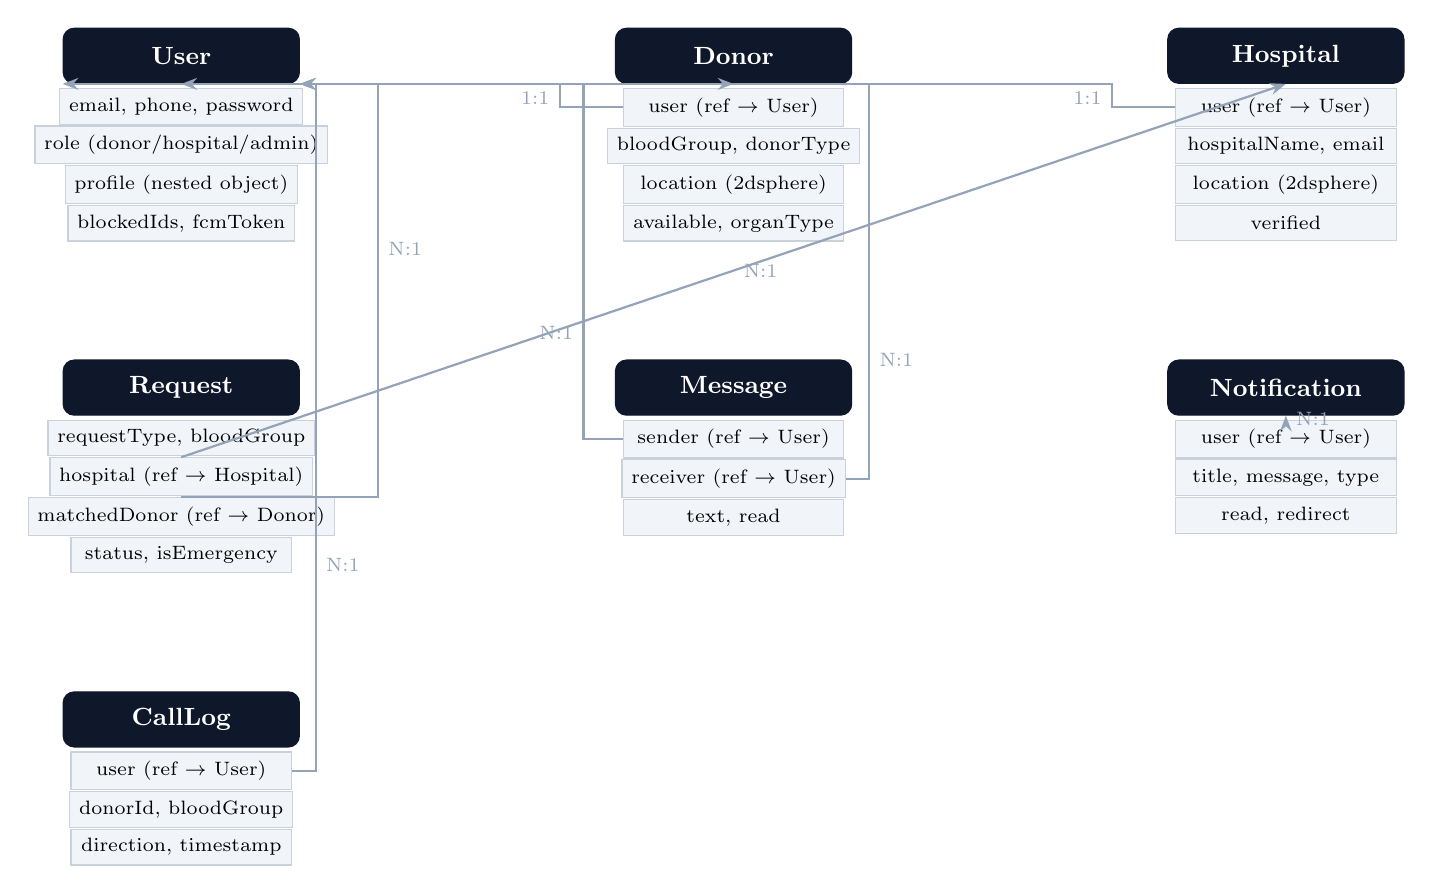
\begin{tikzpicture}[
    entity/.style={rectangle, rounded corners, minimum width=3cm, minimum height=0.7cm, text centered, font=\small\bfseries, fill=dark, text=white, draw=dark},
    attr/.style={rectangle, minimum width=2.8cm, minimum height=0.45cm, text centered, font=\scriptsize, fill=lightgray, draw=midgray!50},
    rel/.style={font=\scriptsize\itseries, text=midgray},
    arr/.style={-{Stealth[length=2mm]}, thick, midgray},
]

% User Entity
\node[entity] (user) {User};
\node[attr, below=0.05cm of user] (u1) {email, phone, password};
\node[attr, below=0.01cm of u1] (u2) {role (donor/hospital/admin)};
\node[attr, below=0.01cm of u2] (u3) {profile (nested object)};
\node[attr, below=0.01cm of u3] (u4) {blockedIds, fcmToken};

% Donor Entity
\node[entity, right=4cm of user] (donor) {Donor};
\node[attr, below=0.05cm of donor] (d1) {user (ref $\rightarrow$ User)};
\node[attr, below=0.01cm of d1] (d2) {bloodGroup, donorType};
\node[attr, below=0.01cm of d2] (d3) {location (2dsphere)};
\node[attr, below=0.01cm of d3] (d4) {available, organType};

% Hospital Entity
\node[entity, right=4cm of donor] (hospital) {Hospital};
\node[attr, below=0.05cm of hospital] (h1) {user (ref $\rightarrow$ User)};
\node[attr, below=0.01cm of h1] (h2) {hospitalName, email};
\node[attr, below=0.01cm of h2] (h3) {location (2dsphere)};
\node[attr, below=0.01cm of h3] (h4) {verified};

% Request Entity
\node[entity, below=3.5cm of user] (request) {Request};
\node[attr, below=0.05cm of request] (r1) {requestType, bloodGroup};
\node[attr, below=0.01cm of r1] (r2) {hospital (ref $\rightarrow$ Hospital)};
\node[attr, below=0.01cm of r2] (r3) {matchedDonor (ref $\rightarrow$ Donor)};
\node[attr, below=0.01cm of r3] (r4) {status, isEmergency};

% Message Entity
\node[entity, right=4cm of request] (message) {Message};
\node[attr, below=0.05cm of message] (m1) {sender (ref $\rightarrow$ User)};
\node[attr, below=0.01cm of m1] (m2) {receiver (ref $\rightarrow$ User)};
\node[attr, below=0.01cm of m2] (m3) {text, read};

% Notification Entity
\node[entity, right=4cm of message] (notif) {Notification};
\node[attr, below=0.05cm of notif] (n1) {user (ref $\rightarrow$ User)};
\node[attr, below=0.01cm of n1] (n2) {title, message, type};
\node[attr, below=0.01cm of n2] (n3) {read, redirect};

% CallLog Entity
\node[entity, below=3.5cm of request] (calllog) {CallLog};
\node[attr, below=0.05cm of calllog] (c1) {user (ref $\rightarrow$ User)};
\node[attr, below=0.01cm of c1] (c2) {donorId, bloodGroup};
\node[attr, below=0.01cm of c2] (c3) {direction, timestamp};

% Relationships
\draw[arr] (d1.west) -- ++(-0.8,0) |- (user.south) node[pos=0.2, rel, left] {1:1};
\draw[arr] (h1.west) -- ++(-0.8,0) |- (user.south east) node[pos=0.2, rel, left] {1:1};
\draw[arr] (r2.north) -- (hospital.south) node[midway, rel, right] {N:1};
\draw[arr] (r3.north) -- ++(2.5,0) |- (donor.south) node[pos=0.3, rel, right] {N:1};
\draw[arr] (m1.west) -- ++(-0.5,0) |- (user.south west) node[pos=0.15, rel, left] {N:1};
\draw[arr] (m2.east) -- ++(0.3,0) |- (user.south east) node[pos=0.15, rel, right] {N:1};
\draw[arr] (n1.north) -- (notif.south) node[pos=0.3, rel, right] {N:1};
\draw[arr] (c1.east) -- ++(0.3,0) |- (user.south east) node[pos=0.15, rel, right] {N:1};

\end{tikzpicture}
\caption{Entity-Relationship Diagram}
\end{figure}

\subsection{Collection Descriptions}

\begin{enumerate}[leftmargin=*]
    \item \textbf{User} --- Core authentication entity. Stores email, phone, hashed password, Google ID, role (donor/hospital/admin), and a nested profile object containing personal, medical, and location data.
    \item \textbf{Donor} --- Extended donor profile linked to User. Contains blood group, organ type, city, phone, geospatial location (2dsphere index), and availability status.
    \item \textbf{Hospital} --- Hospital profile linked to User. Contains hospital name, email, phone, address, geospatial location, and verification status.
    \item \textbf{Request} --- Donation request created by hospitals or users. Contains request type, blood group/organ type, hospital reference, matched donor reference, status (Pending/Matched/Fulfilled), and emergency flags.
    \item \textbf{Message} --- Chat messages between two users. Contains sender, receiver, text content, and read status. Indexed on sender+receiver+createdAt.
    \item \textbf{Notification} --- In-app notifications. Contains user, title, message, type (match/emergency/info/success/error/call), redirect path, and read status.
    \item \textbf{CallLog} --- Records of masked calling sessions. Contains user, donor metadata (blood group, age, gender, city), call type (blood/organ), and direction (incoming/outgoing).
\end{enumerate}

% ══════════════════════════════════════════════════════════════════════════
% SECTION 8: KEY FEATURES
% ══════════════════════════════════════════════════════════════════════════
\section{Key Features}

\subsection{User Registration \& Authentication}

\begin{itemize}[leftmargin=*]
    \item Email + password registration with Joi validation
    \item JWT token-based authentication (30-day expiry)
    \item Google OAuth social login
    \item Password reset flow with OTP verification
    \item Role-based access control (donor, hospital, admin)
\end{itemize}

\subsection{Donor Profile Management}

\begin{itemize}[leftmargin=*]
    \item Complete profile with personal, medical, and location data
    \item Blood group selection from 8 standard groups (A+, A-, B+, B-, AB+, AB-, O+, O-)
    \item Organ donation preferences (Kidney, Liver, Heart, Lungs, Pancreas, Cornea, Bone Marrow)
    \item Medical certificate upload (PDF, PNG, JPG) for eligibility verification
    \item GPS-based or pincode-based location setting
\end{itemize}

\subsection{Smart Donor Search}

\begin{itemize}[leftmargin=*]
    \item Search by blood group or organ type
    \item Filter chips for quick selection
    \item Results sorted by distance using Haversine formula
    \item Blocked donor filtering
    \item Available/Unavailable status display
\end{itemize}

\subsection{Emergency Matching}

\begin{itemize}[leftmargin=*]
    \item Hospitals can mark requests as emergency
    \item Emergency requests notify ALL matching donors in the city
    \item Multi-channel notification: SSE + push notification + email
    \item Urgency levels: low, medium, high, critical
\end{itemize}

\subsection{Real-Time Chat}

\begin{itemize}[leftmargin=*]
    \item Conversation list with unread message counts
    \item Message history with date grouping
    \item Typing indicators
    \item Read receipts (single check / double check)
    \item Online user status
\end{itemize}

\subsection{Masked Calling}

\begin{itemize}[leftmargin=*]
    \item OTP verification before connecting
    \item Both phone numbers remain hidden
    \item Call logging with donor metadata
    \item Re-contact and block functionality
\end{itemize}

\subsection{Notification System}

\begin{itemize}[leftmargin=*]
    \item In-app notification list with read/unread status
    \item Live SSE push for new notifications
    \item Firebase Cloud Messaging for offline push
    \item Mark read, mark all read, clear all
    \item Notification types: match, emergency, info, success, error, call
\end{itemize}

\subsection{Dashboard Analytics}

\begin{itemize}[leftmargin=*]
    \item Total calls, notifications, blood group, donor status cards
    \item Blood search activity bar
    \item Organ match activity bar
    \item Recent activity log
    \item My requests and community requests feed
\end{itemize}

% ══════════════════════════════════════════════════════════════════════════
% SECTION 9: USER FLOW
% ══════════════════════════════════════════════════════════════════════════
\section{User Flow}

\begin{figure}[H]
\centering
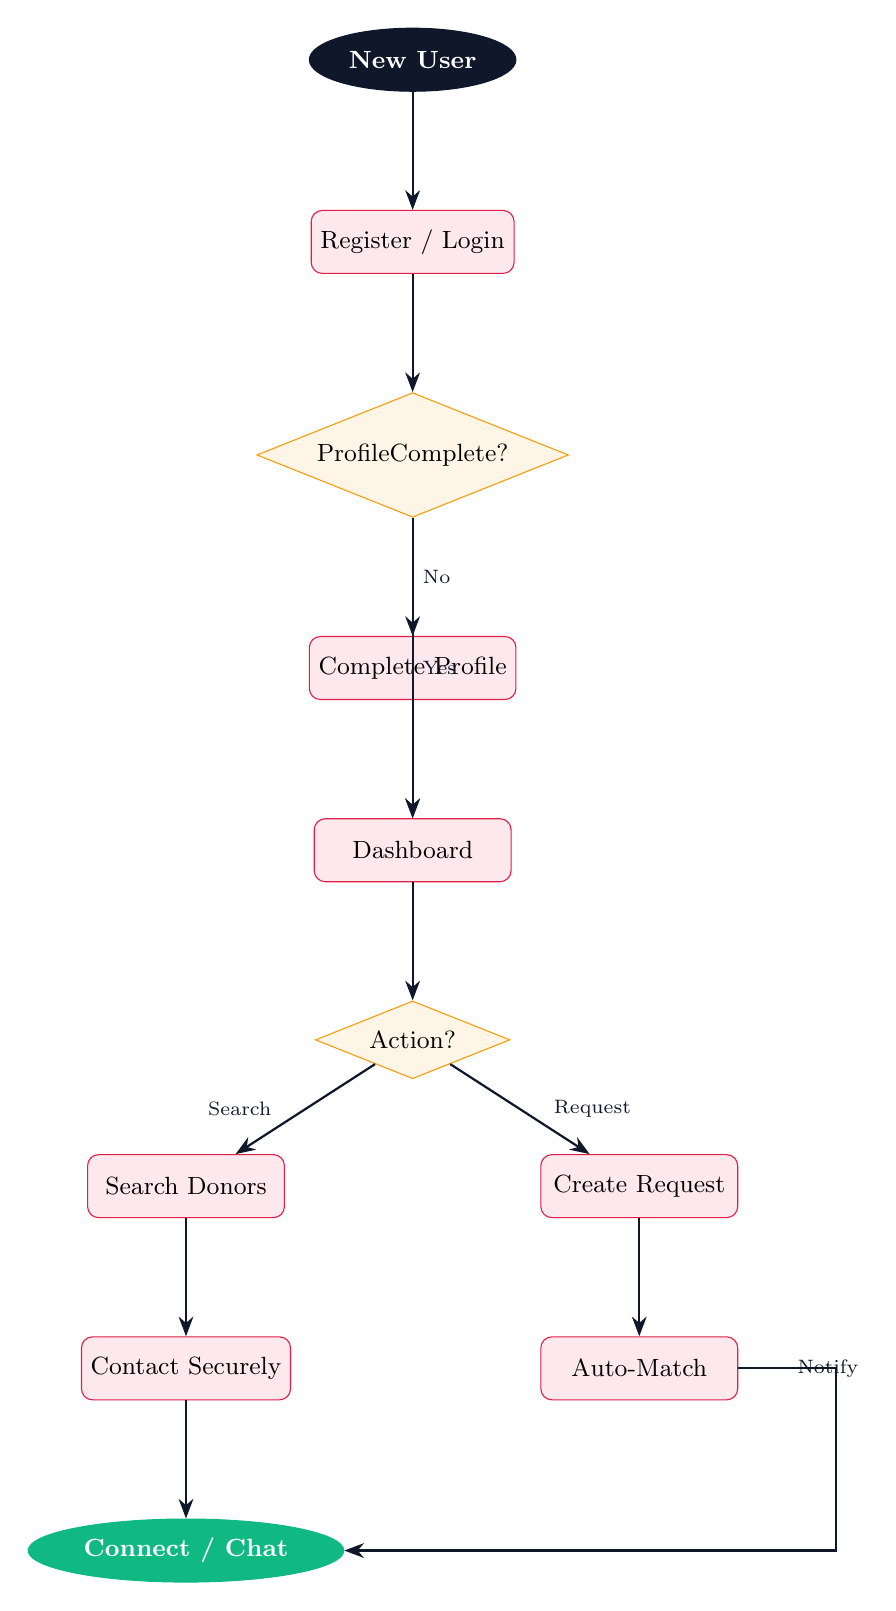
\begin{tikzpicture}[
    node distance=1.5cm,
    start/.style={ellipse, minimum width=2.5cm, minimum height=0.8cm, text centered, font=\small\bfseries, fill=dark, text=white, draw=dark},
    process/.style={rectangle, rounded corners, minimum width=2.5cm, minimum height=0.8cm, text centered, font=\small, fill=primary!10, draw=primary},
    decision/.style={diamond, aspect=2.5, minimum width=2cm, text centered, font=\small, fill=accent!10, draw=accent},
    end/.style={ellipse, minimum width=2cm, minimum height=0.8cm, text centered, font=\small\bfseries, fill=success, text=white, draw=success},
    arr/.style={-{Stealth[length=2.5mm]}, thick, dark},
]

\node[start] (start) {New User};

\node[process, below=of start] (register) {Register / Login};
\node[decision, below=of register] (complete) {Profile\\Complete?};
\node[process, below=of complete] (profile) {Complete Profile};
\node[process, below=of profile] (dashboard) {Dashboard};
\node[decision, below=1.5cm of dashboard] (searchorreq) {Action?};

\node[process, below left=1.2cm and 1cm of searchorreq] (search) {Search Donors};
\node[process, below right=1.2cm and 1cm of searchorreq] (request) {Create Request};
\node[process, below=of search] (contact) {Contact Securely};
\node[process, below=of request] (match) {Auto-Match};
\node[end, below=1.5cm of contact] (connect) {Connect / Chat};

% Arrows
\draw[arr] (start) -- (register);
\draw[arr] (register) -- (complete);
\draw[arr] (complete) -- node[right, font=\scriptsize] {No} (profile);
\draw[arr] (complete) -- node[right, font=\scriptsize] {Yes} (dashboard);
\draw[arr] (profile) -- (dashboard);
\draw[arr] (dashboard) -- (searchorreq);
\draw[arr] (searchorreq) -- node[left, font=\scriptsize, xshift=-0.3cm] {Search} (search);
\draw[arr] (searchorreq) -- node[right, font=\scriptsize, xshift=0.3cm] {Request} (request);
\draw[arr] (search) -- (contact);
\draw[arr] (request) -- (match);
\draw[arr] (contact) -- (connect);
\draw[arr] (match) -- node[right, font=\scriptsize] {Notify} ++(2.5,0) |- (connect);

\end{tikzpicture}
\caption{User Flow Diagram}
\end{figure}

% ══════════════════════════════════════════════════════════════════════════
% SECTION 10: REAL-TIME COMMUNICATION
% ══════════════════════════════════════════════════════════════════════════
\section{Real-Time Communication}

LifeLink uses Server-Sent Events (SSE) for real-time communication between the server and connected clients.

\begin{figure}[H]
\centering
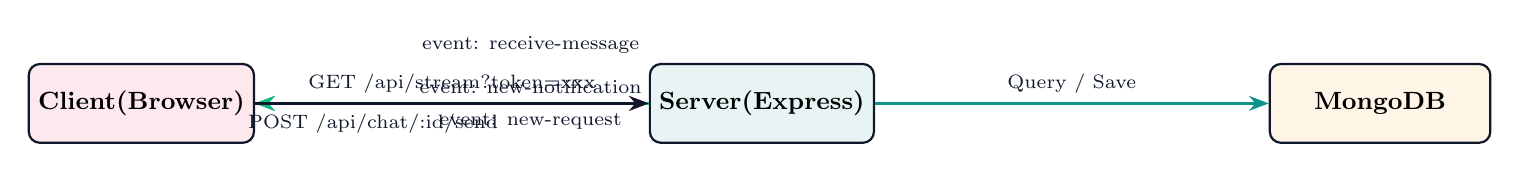
\begin{tikzpicture}[
    node distance=2cm,
    box/.style={rectangle, rounded corners, minimum width=2.8cm, minimum height=1cm, text centered, font=\small\bfseries, draw=dark, line width=0.8pt},
    arr/.style={-{Stealth[length=2.5mm]}, thick},
    evt/.style={font=\scriptsize, text=dark},
]

\node[box, fill=primary!10] (client) {Client\\(Browser)};
\node[box, fill=secondary!10, right=5cm of client] (server) {Server\\(Express)};
\node[box, fill=accent!10, right=5cm of server] (db) {MongoDB};

% Connection
\draw[arr, primary, thick] (client) -- node[above, evt] {GET /api/stream?token=xxx} (server);
\draw[arr, secondary, thick] (server) -- node[above, evt] {Query / Save} (db);

% Events
\draw[arr, success, thick, dashed] (server) to node[above, evt, pos=0.3] {event: new-notification} (client);
\draw[arr, success, thick, dashed] (server) to node[below, evt, pos=0.3] {event: new-request} (client);
\draw[arr, success, thick, dashed] (server) to node[above, evt, pos=0.3, yshift=0.5cm] {event: receive-message} (client);

% REST calls
\draw[arr, dark, thick] (client) to node[below, evt, pos=0.3] {POST /api/chat/:id/send} (server);

\end{tikzpicture}
\caption{Real-Time Communication Flow (SSE)}
\end{figure}

\subsection{SSE Event Types}

\begin{table}[H]
\centering
\renewcommand{\arraystretch}{1.3}
\begin{tabularx}{\textwidth}{|l|X|}
    \hline
    \textbf{Event} & \textbf{Description} \\
    \hline
    connect & Sent on initial SSE connection with status \\
    \hline
    online-users & Broadcasts array of currently online user IDs \\
    \hline
    new-notification & Pushes new notification to specific user \\
    \hline
    new-request & Broadcasts new donation request to all users \\
    \hline
    receive-message & Delivers new chat message to receiver \\
    \hline
    message-sent & Confirms message delivery to sender \\
    \hline
    user-typing & Indicates other user is typing \\
    \hline
    user-stop-typing & Indicates other user stopped typing \\
    \hline
    messages-read & Notifies sender that messages were read \\
    \hline
\end{tabularx}
\caption{SSE Event Types}
\end{table}

\subsection{Connection Resilience}

The SSE connection implements exponential backoff reconnection:
\begin{itemize}[leftmargin=*]
    \item Initial retry: 2 seconds
    \item Each subsequent retry doubles: 2s, 4s, 8s, 16s, 30s (max)
    \item Counter resets on successful connection
    \item Heartbeat every 15 seconds keeps the connection alive
\end{itemize}

% ══════════════════════════════════════════════════════════════════════════
% SECTION 11: DONOR MATCHING ALGORITHM
% ══════════════════════════════════════════════════════════════════════════
\section{Donor Matching Algorithm}

\begin{figure}[H]
\centering
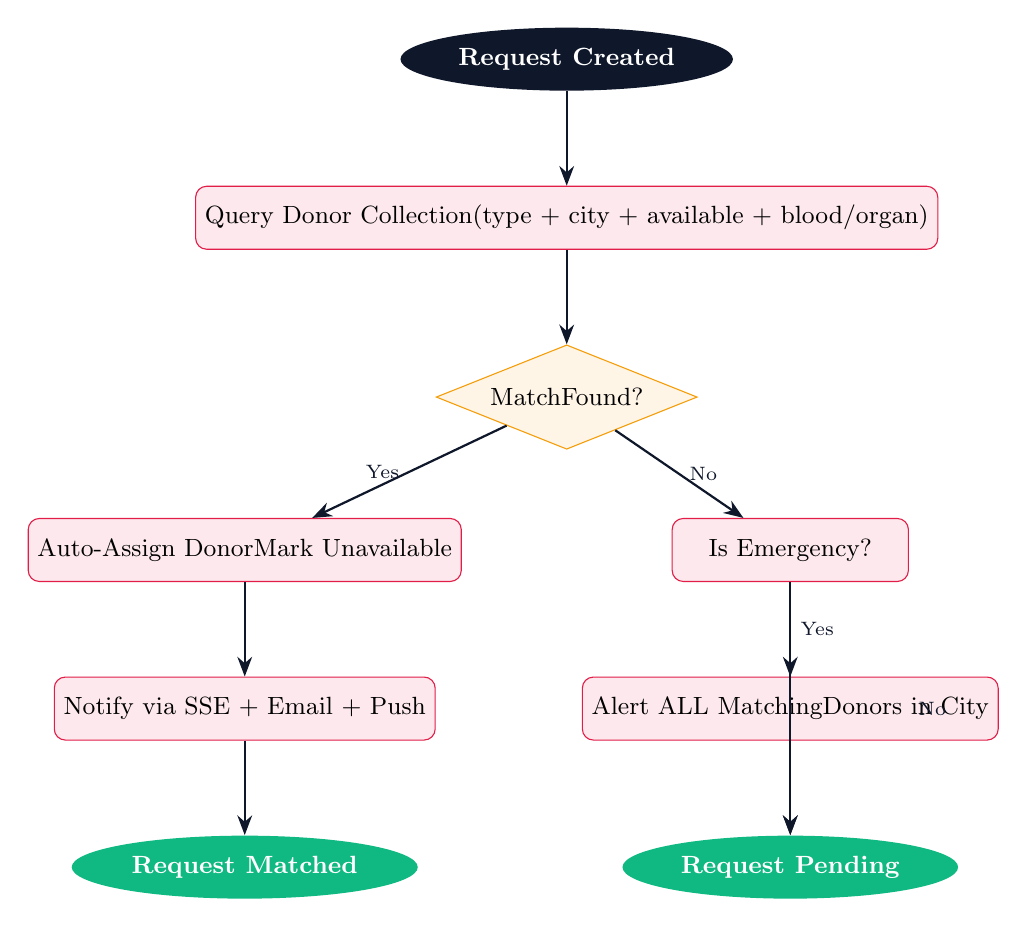
\begin{tikzpicture}[
    node distance=1.2cm,
    start/.style={ellipse, minimum width=2.5cm, minimum height=0.8cm, text centered, font=\small\bfseries, fill=dark, text=white},
    process/.style={rectangle, rounded corners, minimum width=3cm, minimum height=0.8cm, text centered, font=\small, fill=primary!10, draw=primary},
    decision/.style={diamond, aspect=2.5, minimum width=2cm, text centered, font=\small, fill=accent!10, draw=accent},
    end/.style={ellipse, minimum width=2cm, minimum height=0.8cm, text centered, font=\small\bfseries, fill=success, text=white},
    arr/.style={-{Stealth[length=2.5mm]}, thick, dark},
]

\node[start] (start) {Request Created};

\node[process, below=of start] (query) {Query Donor Collection\\(type + city + available + blood/organ)};

\node[decision, below=of query] (found) {Match\\Found?};

\node[process, below left=1.2cm and 0.5cm of found] (assign) {Auto-Assign Donor\\Mark Unavailable};
\node[process, below right=1.2cm and 0.5cm of found] (emergency) {Is Emergency?};

\node[process, below=of assign] (notify) {Notify via SSE + Email + Push};
\node[process, below=of emergency] (alertall) {Alert ALL Matching\\Donors in City};

\node[end, below=of notify] (done) {Request Matched};
\node[end, below=of alertall] (pending) {Request Pending};

\draw[arr] (start) -- (query);
\draw[arr] (query) -- (found);
\draw[arr] (found) -- node[left, font=\scriptsize] {Yes} (assign);
\draw[arr] (found) -- node[right, font=\scriptsize] {No} (emergency);
\draw[arr] (assign) -- (notify);
\draw[arr] (notify) -- (done);
\draw[arr] (emergency) -- node[right, font=\scriptsize] {Yes} (alertall);
\draw[arr] (emergency) -- node[right, font=\scriptsize, xshift=1.5cm] {No} (pending);
\draw[arr] (alertall) -- (pending);

\end{tikzpicture}
\caption{Donor Matching Algorithm Flowchart}
\end{figure}

\subsection{Algorithm Description}

\begin{enumerate}[leftmargin=*]
    \item When a request is created (by hospital or user), the system builds a match query based on request type (blood/organ), city, availability status, and blood group or organ type.
    \item The system queries the Donor collection for the first matching available donor.
    \item \textbf{If a match is found:} The donor is auto-assigned to the request, their availability is set to false, and they are notified via SSE, push notification, and email.
    \item \textbf{If no match is found and it is an emergency:} The system finds ALL available donors in the same city and broadcasts the emergency alert to each of them.
    \item \textbf{If no match and not emergency:} The request stays in Pending status and is visible in the community requests feed.
\end{enumerate}

% ══════════════════════════════════════════════════════════════════════════
% SECTION 12: LOCATION-BASED SEARCH
% ══════════════════════════════════════════════════════════════════════════
\section{Location-Based Search}

\begin{figure}[H]
\centering
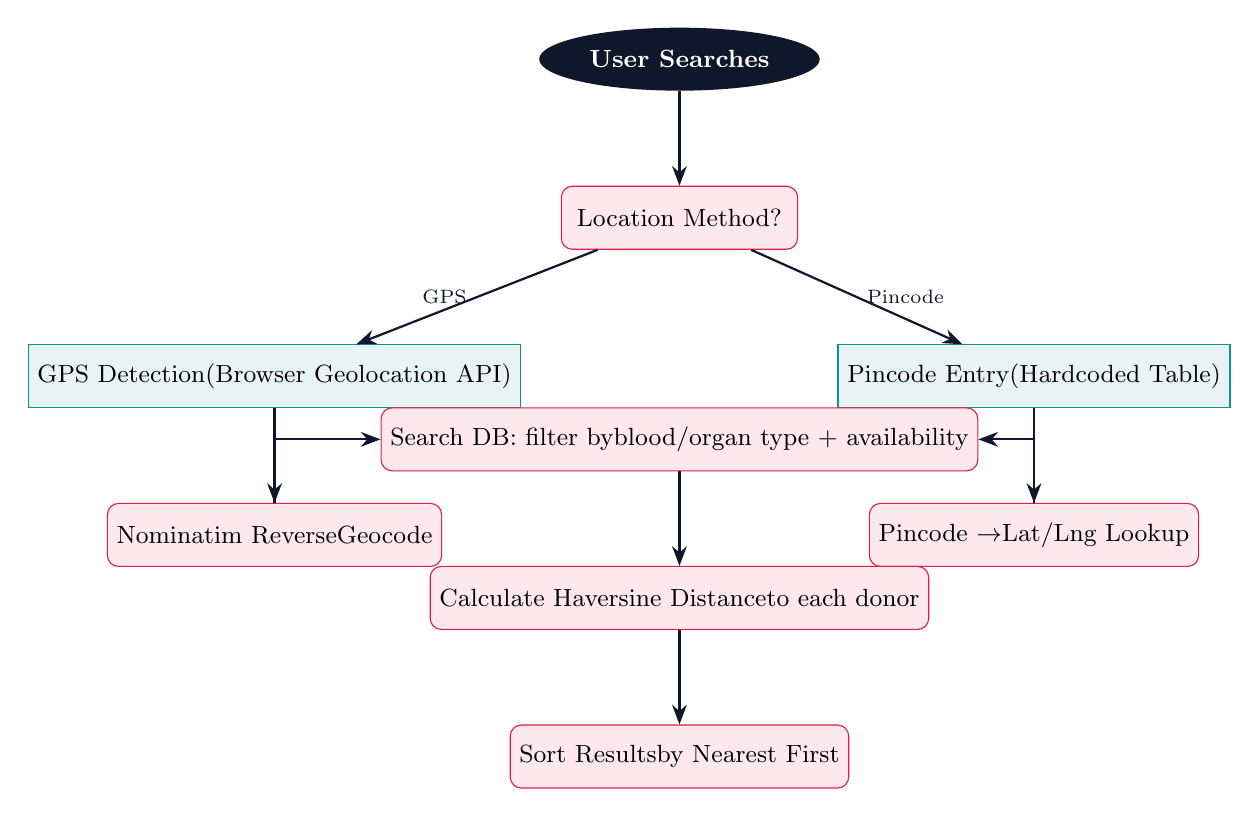
\begin{tikzpicture}[
    node distance=1.2cm,
    start/.style={ellipse, minimum width=2.5cm, minimum height=0.8cm, text centered, font=\small\bfseries, fill=dark, text=white},
    process/.style={rectangle, rounded corners, minimum width=3cm, minimum height=0.8cm, text centered, font=\small, fill=primary!10, draw=primary},
    data/.style={rectangle, minimum width=2.5cm, minimum height=0.8cm, text centered, font=\small, fill=secondary!10, draw=secondary},
    arr/.style={-{Stealth[length=2.5mm]}, thick, dark},
]

\node[start] (start) {User Searches};

\node[process, below=of start] (method) {Location Method?};

\node[data, below left=1.2cm and 0.5cm of method] (gps) {GPS Detection\\(Browser Geolocation API)};
\node[data, below right=1.2cm and 0.5cm of method] (pin) {Pincode Entry\\(Hardcoded Table)};

\node[process, below=of gps] (reverse) {Nominatim Reverse\\Geocode};
\node[process, below=of pin] (lookup) {Pincode $\rightarrow$\\Lat/Lng Lookup};

\node[process, below=2cm of method] (search) {Search DB: filter by\\blood/organ type + availability};
\node[process, below=of search] (haversine) {Calculate Haversine Distance\\to each donor};
\node[process, below=of haversine] (sort) {Sort Results\\by Nearest First};

\draw[arr] (start) -- (method);
\draw[arr] (method) -- node[left, font=\scriptsize] {GPS} (gps);
\draw[arr] (method) -- node[right, font=\scriptsize] {Pincode} (pin);
\draw[arr] (gps) -- (reverse);
\draw[arr] (pin) -- (lookup);
\draw[arr] (reverse) |- (search);
\draw[arr] (lookup) |- (search);
\draw[arr] (search) -- (haversine);
\draw[arr] (haversine) -- (sort);

\end{tikzpicture}
\caption{Location-Based Search Flowchart}
\end{figure}

\subsection{Haversine Formula}

The Haversine formula calculates the great-circle distance between two points on Earth given their latitude and longitude:

\[
d = 2R \cdot \arcsin\left(\sqrt{\sin^2\left(\frac{\Delta\phi}{2}\right) + \cos(\phi_1) \cdot \cos(\phi_2) \cdot \sin^2\left(\frac{\Delta\lambda}{2}\right)}\right)
\]

Where:
\begin{itemize}[leftmargin=*]
    \item $R$ = Earth's radius (6371 km)
    \item $\phi_1, \phi_2$ = latitudes of the two points (in radians)
    \item $\Delta\phi$ = difference in latitude
    \item $\Delta\lambda$ = difference in longitude
\end{itemize}

\subsection{Location Sources}

\begin{enumerate}[leftmargin=*]
    \item \textbf{GPS (Primary)} --- Uses the browser's Geolocation API to get latitude/longitude, then calls Nominatim (OpenStreetMap) for reverse geocoding to get city name and pincode.
    \item \textbf{Pincode (Fallback)} --- A hardcoded lookup table maps 10 Indian city pincodes to coordinates. Default: Pune (18.5204, 73.8567).
\end{enumerate}

% ══════════════════════════════════════════════════════════════════════════
% SECTION 13: SECURITY IMPLEMENTATION
% ══════════════════════════════════════════════════════════════════════════
\section{Security Implementation}

\begin{figure}[H]
\centering
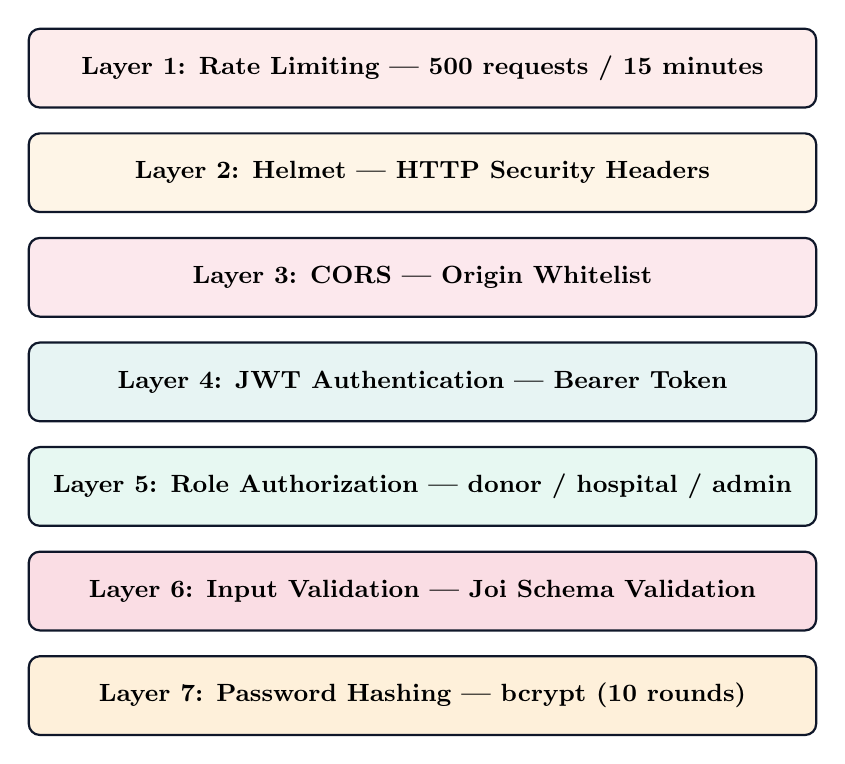
\begin{tikzpicture}[
    node distance=1cm,
    layer/.style={rectangle, rounded corners, minimum width=10cm, minimum height=1cm, text centered, font=\small\bfseries, draw=dark, line width=0.8pt},
    arr/.style={-{Stealth[length=2mm]}, thick, dark},
]

\node[layer, fill=danger!10] (l1) {Layer 1: Rate Limiting --- 500 requests / 15 minutes};
\node[layer, fill=accent!10, below=0.3cm of l1] (l2) {Layer 2: Helmet --- HTTP Security Headers};
\node[layer, fill=primary!10, below=0.3cm of l2] (l3) {Layer 3: CORS --- Origin Whitelist};
\node[layer, fill=secondary!10, below=0.3cm of l3] (l4) {Layer 4: JWT Authentication --- Bearer Token};
\node[layer, fill=success!10, below=0.3cm of l4] (l5) {Layer 5: Role Authorization --- donor / hospital / admin};
\node[layer, fill=primary!15, below=0.3cm of l5] (l6) {Layer 6: Input Validation --- Joi Schema Validation};
\node[layer, fill=accent!15, below=0.3cm of l6] (l7) {Layer 7: Password Hashing --- bcrypt (10 rounds)};

\end{tikzpicture}
\caption{Security Layers Diagram}
\end{figure}

\subsection{Security Measures}

\begin{enumerate}[leftmargin=*]
    \item \textbf{Rate Limiting} --- Express rate limiter restricts API to 500 requests per 15 minutes per IP, preventing brute-force and DDoS attacks.
    \item \textbf{HTTP Security Headers} --- Helmet middleware adds security headers like Content-Security-Policy, X-Frame-Options, and HSTS.
    \item \textbf{CORS Configuration} --- Only whitelisted origins (localhost:5173, production domain) can make cross-origin requests.
    \item \textbf{JWT Authentication} --- Stateless token-based auth. Tokens expire after 30 days. Protected routes verify the Bearer token on every request.
    \item \textbf{Role-Based Access Control} --- Three roles: donor, hospital, admin. Hospital-only routes (like creating requests) are protected by role middleware.
    \item \textbf{Input Validation} --- Joi schemas validate all incoming request bodies for register, login, and password reset.
    \item \textbf{Password Hashing} --- bcrypt with 10 salt rounds. Raw passwords are never stored.
    \item \textbf{Privacy} --- Donor cards never display name, phone, or email. Only age, gender, blood group, weight, and city are shown.
    \item \textbf{Account Deletion} --- Requires password confirmation. Associated call logs and notifications are also deleted.
    \item \textbf{Donor Blocking} --- Users can block specific donors. Blocked IDs are stored per user and filtered from search results.
\end{enumerate}

% ══════════════════════════════════════════════════════════════════════════
% SECTION 14: DEPLOYMENT
% ══════════════════════════════════════════════════════════════════════════
\section{Deployment Architecture}

\begin{figure}[H]
\centering
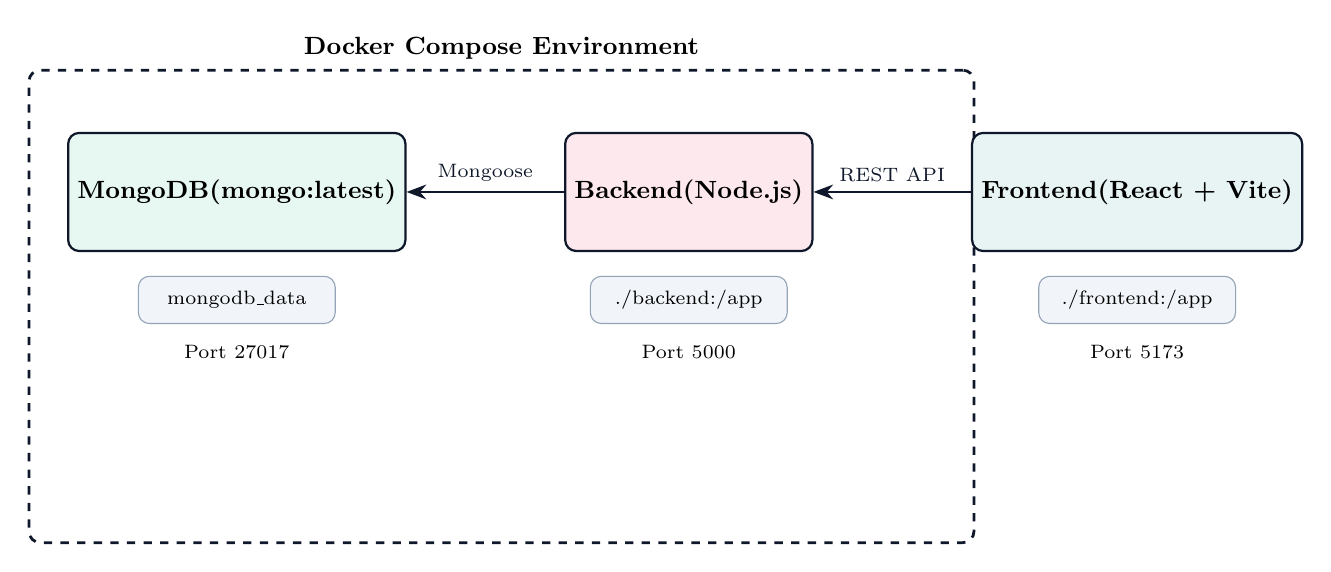
\begin{tikzpicture}[
    node distance=2cm,
    container/.style={rectangle, rounded corners, minimum width=3cm, minimum height=1.5cm, text centered, font=\small\bfseries, draw=dark, line width=0.8pt},
    vol/.style={rectangle, rounded corners, minimum width=2.5cm, minimum height=0.6cm, text centered, font=\scriptsize, fill=lightgray, draw=midgray},
    arr/.style={-{Stealth[length=2.5mm]}, thick, dark},
]

% Docker Host
\node[rectangle, rounded corners, draw=dark, line width=1pt, dashed, minimum width=12cm, minimum height=6cm, label={[font=\bfseries\small]Docker Compose Environment}] (docker) {};

% Containers
\node[container, fill=success!10, below right=0.8cm and 0.5cm of docker.north west] (mongo) {MongoDB\\(mongo:latest)};
\node[container, fill=primary!10, right=2cm of mongo] (backend) {Backend\\(Node.js)};
\node[container, fill=secondary!10, right=2cm of backend] (frontend) {Frontend\\(React + Vite)};

% Volumes
\node[vol, below=0.3cm of mongo] (vol1) {mongodb\_data};
\node[vol, below=0.3cm of backend] (vol2) {./backend:/app};
\node[vol, below=0.3cm of frontend] (vol3) {./frontend:/app};

% Ports
\node[font=\scriptsize, below=0.15cm of vol1] {Port 27017};
\node[font=\scriptsize, below=0.15cm of vol2] {Port 5000};
\node[font=\scriptsize, below=0.15cm of vol3] {Port 5173};

% Arrows
\draw[arr] (backend) -- node[above, font=\scriptsize] {Mongoose} (mongo);
\draw[arr] (frontend) -- node[above, font=\scriptsize] {REST API} (backend);

\end{tikzpicture}
\caption{Docker Compose Deployment Architecture}
\end{figure}

\subsection{Deployment Configuration}

\begin{table}[H]
\centering
\renewcommand{\arraystretch}{1.3}
\begin{tabularx}{\textwidth}{|l|X|X|}
    \hline
    \textbf{Service} & \textbf{Configuration} & \textbf{Details} \\
    \hline
    MongoDB & mongo:latest image & Persistent volume, port 27017 \\
    \hline
    Backend & Custom Dockerfile & Port 5000, env from .env file, depends on MongoDB \\
    \hline
    Frontend & Custom Dockerfile & Port 5173, Vite dev server, depends on Backend \\
    \hline
\end{tabularx}
\caption{Docker Compose Service Configuration}
\end{table}

\subsection{Environment Variables}

\begin{table}[H]
\centering
\renewcommand{\arraystretch}{1.3}
\begin{tabularx}{\textwidth}{|l|X|}
    \hline
    \textbf{Variable} & \textbf{Purpose} \\
    \hline
    MONGO\_URI & MongoDB Atlas connection string \\
    \hline
    JWT\_SECRET & Secret key for JWT token signing \\
    \hline
    GOOGLE\_CLIENT\_ID & Google OAuth client ID \\
    \hline
    PORT & Backend server port (5000) \\
    \hline
    NODE\_ENV & Environment mode (development/production) \\
    \hline
    VITE\_API\_URL & Frontend API base URL \\
    \hline
    VITE\_GOOGLE\_CLIENT\_ID & Google OAuth client ID for frontend \\
    \hline
\end{tabularx}
\caption{Key Environment Variables}
\end{table}

% ══════════════════════════════════════════════════════════════════════════
% SECTION 15: FRONTEND ARCHITECTURE
% ══════════════════════════════════════════════════════════════════════════
\section{Frontend Architecture}

\begin{figure}[H]
\centering
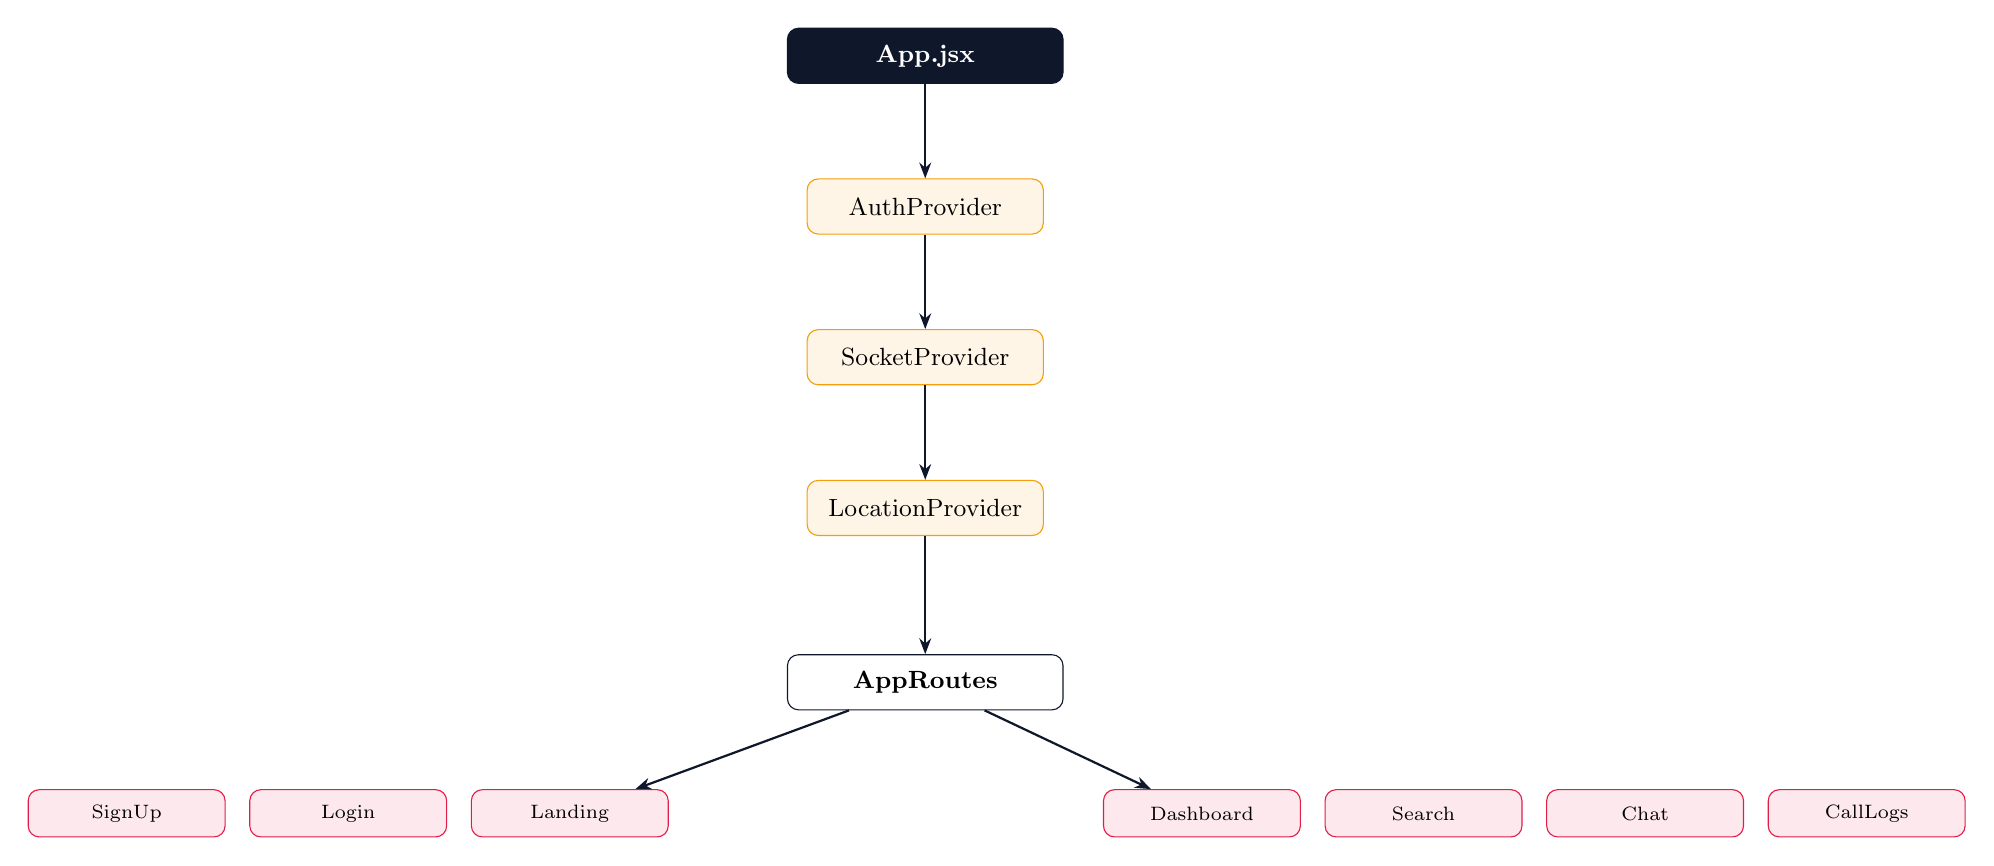
\begin{tikzpicture}[
    node distance=1.2cm,
    comp/.style={rectangle, rounded corners, minimum width=3.5cm, minimum height=0.7cm, text centered, font=\small\bfseries, draw=dark},
    ctx/.style={rectangle, rounded corners, minimum width=3cm, minimum height=0.7cm, text centered, font=\small, fill=accent!10, draw=accent},
    page/.style={rectangle, rounded corners, minimum width=2.5cm, minimum height=0.6cm, text centered, font=\scriptsize, fill=primary!10, draw=primary},
    arr/.style={-{Stealth[length=2mm]}, thick, dark},
]

% App Root
\node[comp, fill=dark, text=white] (app) {App.jsx};

% Providers
\node[ctx, below=of app] (auth) {AuthProvider};
\node[ctx, below=of auth] (socket) {SocketProvider};
\node[ctx, below=of socket] (loc) {LocationProvider};

% Routes
\node[comp, below=1.5cm of loc] (routes) {AppRoutes};

% Public Pages
\node[page, below left=1cm and 1.5cm of routes] (landing) {Landing};
\node[page, left=0.3cm of landing] (login) {Login};
\node[page, left=0.3cm of login] (signup) {SignUp};

% Protected Pages
\node[page, below right=1cm and 0.5cm of routes] (dashboard) {Dashboard};
\node[page, right=0.3cm of dashboard] (search) {Search};
\node[page, right=0.3cm of search] (chat) {Chat};
\node[page, right=0.3cm of chat] (calls) {CallLogs};

% Arrows
\draw[arr] (app) -- (auth);
\draw[arr] (auth) -- (socket);
\draw[arr] (socket) -- (loc);
\draw[arr] (loc) -- (routes);
\draw[arr] (routes) -- (landing);
\draw[arr] (routes) -- (dashboard);

\end{tikzpicture}
\caption{Frontend Component Hierarchy}
\end{figure}

\subsection{Context Providers}

\begin{enumerate}[leftmargin=*]
    \item \textbf{AuthProvider} --- Manages user state, authentication (login, signup, logout, Google auth), profile updates, notifications, call logs, and blocked donors.
    \item \textbf{SocketProvider} --- Manages SSE connection to the server. Provides socket shim for chat events, online user status, and reconnection logic.
    \item \textbf{LocationProvider} --- Manages GPS detection (via Nominatim reverse geocode) and pincode-based location setting.
\end{enumerate}

\subsection{Route Protection}

\begin{itemize}[leftmargin=*]
    \item \textbf{ProtectedRoute} --- Redirects to /login if user is not authenticated
    \item \textbf{PublicOnlyRoute} --- Redirects to /dashboard if user is already authenticated
    \item Dashboard routes are nested inside DashboardLayout with sidebar navigation
\end{itemize}

% ══════════════════════════════════════════════════════════════════════════
% SECTION 16: API ENDPOINTS
% ══════════════════════════════════════════════════════════════════════════
\section{API Endpoints}

\begin{table}[H]
\centering
\renewcommand{\arraystretch}{1.2}
\scriptsize
\begin{tabularx}{\textwidth}{|l|l|X|l|}
    \hline
    \textbf{Method} & \textbf{Route} & \textbf{Description} & \textbf{Auth} \\
    \hline
    POST & /api/auth/register & Register new user & Public \\
    \hline
    POST & /api/auth/login & Login with credentials & Public \\
    \hline
    POST & /api/auth/google & Google OAuth login & Public \\
    \hline
    POST & /api/auth/reset-password & Reset password & Public \\
    \hline
    GET & /api/auth/me & Get current user & Private \\
    \hline
    PUT & /api/auth/profile & Update profile & Private \\
    \hline
    POST & /api/auth/delete & Delete account & Private \\
    \hline
    POST & /api/auth/block/:id & Block donor & Private \\
    \hline
    POST & /api/auth/unblock/:id & Unblock donor & Private \\
    \hline
    POST & /api/auth/fcm-token & Save FCM token & Private \\
    \hline
    POST & /api/requests & Create hospital request & Hospital \\
    \hline
    GET & /api/requests & Get all requests & Private \\
    \hline
    GET & /api/requests/mine & Get my requests & Private \\
    \hline
    POST & /api/requests/donor & Create donor request & Private \\
    \hline
    PATCH & /api/requests/:id & Update request status & Hospital \\
    \hline
    GET & /api/search & Search donors & Optional \\
    \hline
    GET & /api/search/:id & Get donor by ID & Private \\
    \hline
    GET & /api/chat & Get chat list & Private \\
    \hline
    GET & /api/chat/:id & Get chat history & Private \\
    \hline
    POST & /api/chat/:id/send & Send message & Private \\
    \hline
    POST & /api/chat/:id/read & Mark messages read & Private \\
    \hline
    POST & /api/chat/:id/typing & Send typing indicator & Private \\
    \hline
    GET & /api/notifications & Get notifications & Private \\
    \hline
    PATCH & /api/notifications/:id/read & Mark as read & Private \\
    \hline
    POST & /api/notifications/read-all & Mark all read & Private \\
    \hline
    DELETE & /api/notifications & Clear all & Private \\
    \hline
    GET & /api/calls & Get call logs & Private \\
    \hline
    POST & /api/calls & Add call log & Private \\
    \hline
    DELETE & /api/calls/:id & Delete call log & Private \\
    \hline
    GET & /api/dashboard/stats & Get KPI stats & Public \\
    \hline
    GET & /api/dashboard/blood-distribution & Blood group distribution & Public \\
    \hline
    GET & /api/dashboard/monthly-trends & Monthly request trends & Public \\
    \hline
    GET & /api/stream & SSE event stream & Token \\
    \hline
\end{tabularx}
\caption{Complete API Endpoint Reference}
\end{table}

% ══════════════════════════════════════════════════════════════════════════
% SECTION 17: LIMITATIONS
% ══════════════════════════════════════════════════════════════════════════
\section{Limitations}

\begin{enumerate}[leftmargin=*]
    \item \textbf{OTP is Demo Only} --- The OTP verification uses a hardcoded value (123456). No real SMS or email service is integrated.
    \item \textbf{Medical Verification is Simulated} --- The eligibility verification checks the uploaded filename for keywords rather than actually verifying the certificate content.
    \item \textbf{No Actual Phone Calling} --- The masked calling feature simulates a call with a timer. No actual phone connection is established.
    \item \textbf{Base64 File Storage} --- Medical certificates are stored as base64 strings in MongoDB, which is not scalable for large files.
    \item \textbf{Limited Pincode Database} --- Only 10 Indian city pincodes are hardcoded in the location lookup table.
    \item \textbf{No Email Service Configured} --- Nodemailer is configured but no SMTP credentials are provided, so emails are not actually sent.
\end{enumerate}

% ══════════════════════════════════════════════════════════════════════════
% SECTION 18: FUTURE SCOPE
% ══════════════════════════════════════════════════════════════════════════
\section{Future Scope}

\begin{enumerate}[leftmargin=*]
    \item \textbf{Real OTP Integration} --- Integrate Twilio or MSG91 for actual SMS-based OTP verification.
    \item \textbf{Real Phone Calling} --- Implement WebRTC or Twilio for actual masked voice calls.
    \item \textbf{AI-Based Donor Recommendation} --- Use machine learning to predict donor availability and recommend optimal matches.
    \item \textbf{Mobile Application} --- Build a React Native mobile app for Android and iOS.
    \item \textbf{Government Integration} --- Integrate with national health databases for verified donor records.
    \item \textbf{Multi-Language Support} --- Add support for regional Indian languages.
    \item \textbf{Real Medical Verification} --- Implement OCR or AI-based certificate verification.
    \item \textbf{Video Calling} --- Add WebRTC-based video consultation between donors and hospitals.
    \item \textbf{International Expansion} --- Extend the platform globally with multi-country support.
    \item \textbf{Blockchain Verification} --- Use blockchain for tamper-proof donor verification records.
\end{enumerate}

% ══════════════════════════════════════════════════════════════════════════
% SECTION 19: CONCLUSION
% ══════════════════════════════════════════════════════════════════════════
\section{Conclusion}

LifeLink successfully demonstrates a complete web-based blood and organ donor matching system. The platform provides:

\begin{itemize}[leftmargin=*]
    \item A \textbf{centralized donor database} with verified profiles
    \item \textbf{Real-time search} using location-based algorithms
    \item \textbf{Automated matching} that pairs requests with available donors
    \item \textbf{Secure communication} through chat and masked calling
    \item \textbf{Privacy-first design} that protects user identities
    \item \textbf{Emergency support} with instant city-wide alerts
\end{itemize}

The system is built using modern web technologies (MERN stack) with real-time capabilities (SSE) and is containerized for easy deployment. While certain features like OTP verification and phone calling are currently simulated, the core architecture supports future integration with real services.

LifeLink represents a step toward technology-driven healthcare solutions that can save lives by reducing the time gap between those who need donations and those who can provide them.

% ══════════════════════════════════════════════════════════════════════════
% REFERENCES
% ══════════════════════════════════════════════════════════════════════════
\newpage
\section*{References}
\addcontentsline{toc}{section}{References}

\begin{enumerate}[leftmargin=*]
    \item MongoDB Documentation. \url{https://docs.mongodb.com/}
    \item Express.js Documentation. \url{https://expressjs.com/}
    \item React Documentation. \url{https://react.dev/}
    \item Node.js Documentation. \url{https://nodejs.org/en/docs/}
    \item Firebase Cloud Messaging. \url{https://firebase.google.com/docs/cloud-messaging}
    \item Server-Sent Events (MDN). \url{https://developer.mozilla.org/en-US/docs/Web/API/Server-sent_events}
    \item Haversine Formula. \url{https://en.wikipedia.org/wiki/Haversine_formula}
    \item Nominatim (OpenStreetMap). \url{https://nominatim.openstreetmap.org/}
    \item Socket.IO Documentation. \url{https://socket.io/}
    \item Docker Compose Documentation. \url{https://docs.docker.com/compose/}
\end{enumerate}

\end{document}
